\documentclass[12pt]{article}

\usepackage{hyperref}
\usepackage[utf8x]{inputenc}
\usepackage{graphicx,url}
\usepackage{longtable,tabu}
\usepackage[brazil]{babel}   
\usepackage[sort,comma]{natbib}
\usepackage{url} % Provides better formatting of URLs.
\usepackage{hyperref}
\usepackage{geometry}
\geometry{a4paper,total={150mm,237mm},left=30mm,top=35mm}
\pagestyle{plain}
\pagenumbering{arabic}

\sloppy

\begin{document} 
	\title{Uma Análise Ética da Tecnologia Automotiva e suas Consequências: Como especular os impactos, aplicações e implicações dessa insurgente tecnologia na sociedade}
	
	\author{Guilherme Mendel de Almeida Nascimento}
	
	\renewcommand{\tablename}{Quadro}
	
	\newcommand{\address}{
			\begin{center}
				\footnotesize
				Universidade de Brasília - Instituto de Ciências Exatas\\  Departamento de Ciência da Computação - CIC 116726 - Informática e Sociedade \\
				2017.2 - Turma B - Professor Jorge Henrique Cabral Fernandes\\ Prédio CIC/EST - Campus Universitário Darcy Ribeiro \\Asa Norte 70919-970 Brasília, DF\\
				\href{mailto:guimendeln@gmail.com}{guimendeln@gmail.com}
			\end{center}
	}
	
	\maketitle
	\address
	
	\begin{abstract} 
		O artigo, relacionado à tecnologia automotiva aplicada em carros, levanta questões éticas, sociais, econômicas e jurídicas referentes à implementação dessa tecnologia revolucionária no mercado. Traz exemplos da sua aplicação já atualmente, como o projeto da Universidade de Oxford, o Robotcar. A análise engobla o debate carro independente - carro conectado, apresentando diferentes pontos de vista e avaliando as respectivas vantagens e desvantagens de cada.
		
		\textbf{Palavras-chave:} \textit{Informática e Sociedade. UnB. ABNT 10719. Artigo Científico. Carros autônomos. Ética computacional.}
	\end{abstract}
	
	\section{Introdução}
	
		A utilização de robôs na vida rotineira ja foi tema de filmes de ficção científica na década de 90, e as pessoas especulavam largamente sobre quais seriam suas aplicações e usos, apesar de preferir mais se divertir imaginando o mundo dominado por eles. No entanto, hodiernamente, a presença desses robôs já se faz constante em indústrias, empresas de alto rendimento e até mesmo alguns domicílios. O propósito desse artigo é estimular o debate acerca da atuação desses robôs na área automotiva, na forma de carros inteligentes, capazes de dirigir por si próprios, e introduzir alguns modelos teóricos ou ainda reais de como eles poderiam ser implementados.
		
		O artigo \emph{``The Ethics of Driverless Cars"}, de \citet{mcbride_ethics_2016}, empregado como base deste, utiliza-se do projeto RobotCar, da \citet{oxford_robotics_institute_robotcar_nodate}, na construção de sua crítica. Dividido em 6 seções e conclusão final, contrasta, sobretudo, a contraposição de carros, um completamente independente e outro completamente conectado, ambos automotivos, porém opostos em funcionamento.
		
	\section{\label{metodologia}Metodologia} 
		
		Ao longo deste trabalho, serão utilizadas referências, sobretudo, a dois outros artigos:
		\begin{itemize}
			\item \emph{``The Ethics of Driverless Cars"} \citep{mcbride_ethics_2016}, já supracitado, que servirá como alicerce para o desenvolvimento de argumentos e críticas.
			\item \emph{``Doing the right thing: computer ethics pedagogy revisited"} \citep{jones_doing_2016}, que busca revisar e propor uma alternativa acerca dos aspectos gerais presentes na metodologia base que vem sendo utilizada em massa no estudo da ética computacional. A metodologia proposta consiste na análise de casos específicos de estudo em 6 passos, a saber:
			\begin{enumerate}
				\item Identificar os principais dilemas éticos que entram em jogo e o caso de ICTs envolvido;
				\item Compreender o contexto social do design, implementação e uso, realizando uma análise afundo, das tecnologias específicas envolvidas;
				\item Identificar explicitamente todos os valores e princípios, morais e éticos, relevantes ao caso em questão, e especular exemplos práticos que possam demonstrar o conflito desses valores;
				\item Considerar leis (existentes ou implementáveis) que possam ser levantadas nesse contexto, salientar questões na área de jurisdição legal, abordar pontenciais interesses políticos e econômicos por trás de uma eventual lei;
				\item Os 3 últimos são revisitados de maneira a estipular uma conduta aplicável profissionalmente, considerando, por exemplo, as politicas e códigos de organizações privadas e públicas.
				\item Avaliar todas as potenciais soluções e cursos de ação práticos.
			\end{enumerate}
		O artigo seguirá a lógica desses 6 momentos, além de aventar exemplos didáticos e referências, de modo a facilitar a visualização do tema abordado.
		\end{itemize}
		
	\section{\label{dilemas:eticos}Dilemas éticos}
		
		O artigo de \citet{mcbride_ethics_2016} faz uma reflexão ética sobretudo em relação ao tema autonomia, no qual o usuário da tecnologia a cede para o veículo, que se torna então responsável pela trajetória.
		
		Afinal, o que mais pesa nessa troca: a soberania e capacidade de decisão do indivíduo ou a conveniência e segurança ofertadas pelo carro autônomo? O autor reforça a necessidade de mudança no sistema de transporte atual, por razões como congestionamento, poluição e acidentes, e que, para atingir essa mudança, é necessária a integração da rede de sistemas e da comunidade. Mas permanece a dúvida - seria esse realmente um passo na direção certa?
		
		O potencial cliente e consumidor desse novo produto seria, mais do que um governo ou uma empresa, deparado com essa complicada questão. Afinal ainda hoje existem dilemas cuja escolha parte mais da opinião individual de cada um do que de um conceito geral de certo e errado, como é o caso da legalização do porte de armas, da venda de algumas drogas, ou mais ainda, do aborto e do sistema de cotas.
		
		E mais: se uma fabricante escolher o carro autônomo, dever-se-ia optar pelo independente, capaz de se isolar do mundo e aprender com sua experiência, por meio de Machine Learning; ou pelo conectado, totalmente integrado ao mundo ao seu redor e à internet das coisas?
		
	\section{\label{tecnologica}Análise tecnológica}
	
		Existe uma série de tecnologias que podem ser relacionadas a essa em questão. Vale a pena ressaltar algumas a ela mais impactantes e mais próximas.
		
		
		\subsection{RobotCar}
		\begin{figure}[ht]
			\centering
			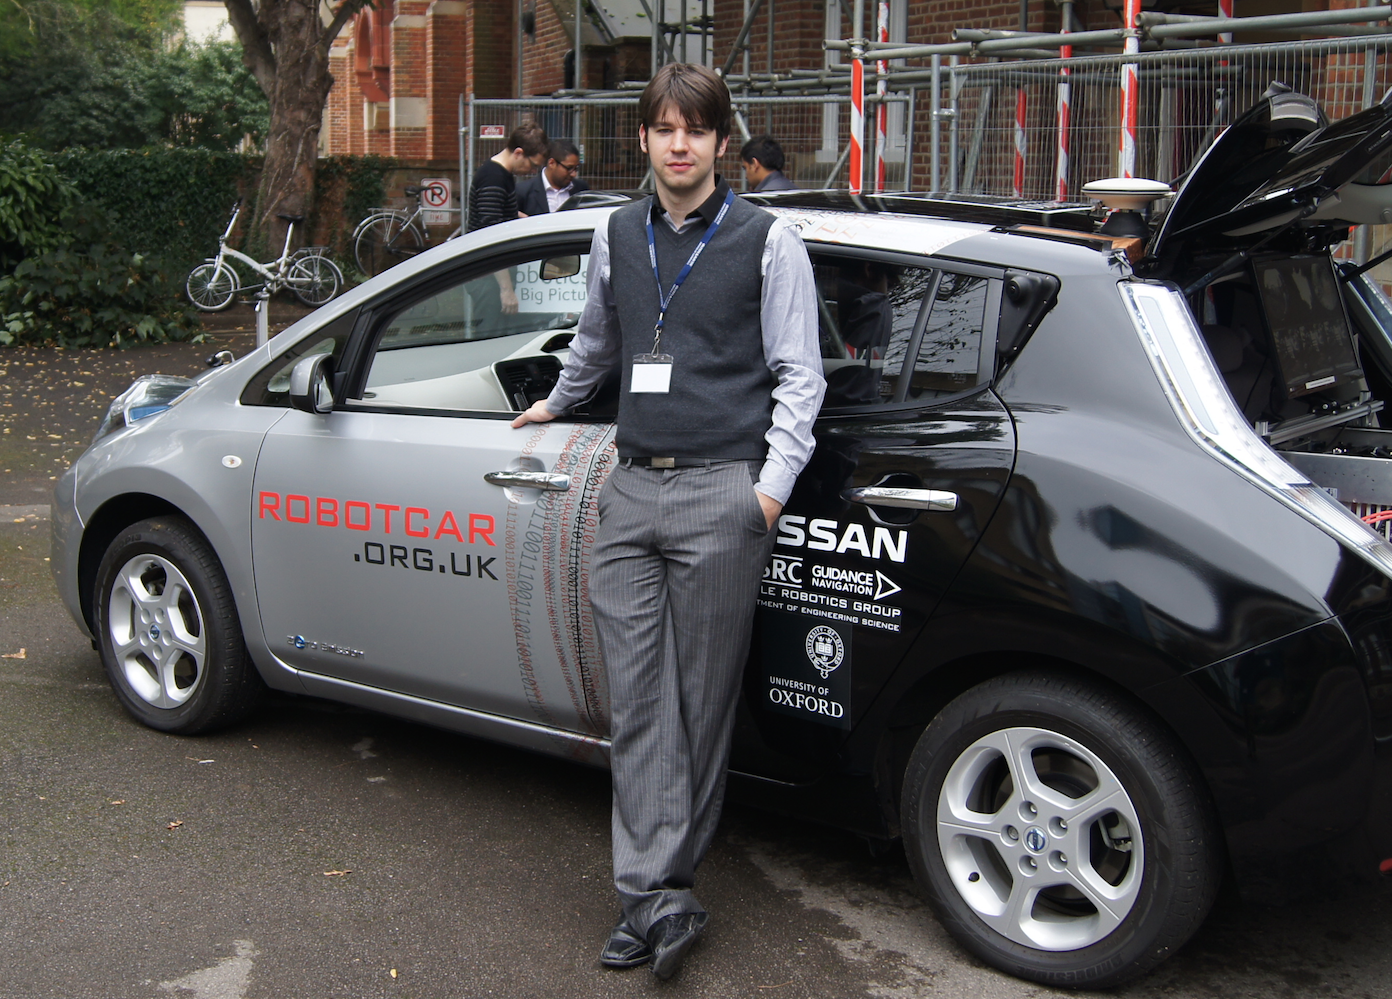
\includegraphics[width=.85\textwidth]{will-robotcar.png}
			\caption{Will Maddern e um protótipo do RobotCar. Fonte: Oxford Robotics Institute, internet. }\label{fig:1}
		\end{figure}
		Uma das tecnologias envolvidas no debate, que pode servir de exemplo, é o próprio RobotCar \citep{oxford_robotics_institute_robotcar_nodate}, um projeto em desenvolvimento por um grupo acadêmico do Instituto de Robótica de Oxford (ORI). Seu objetivo é resumido em \emph{“(…) extender o alcance da navegação automática para escalas efetivamente vastas sem necessitar de modificações do ambiente tão caras, desajeitadas e inconvenientes. É sobre abrir portas para que as máquinas operem para nós, conosco e ao nosso lado na multitude de espaços em que habitamos, frequentamos e nos quais trabalhamos.”}, o que indica que o carro seria capaz de se conduzir livremente em quase qualquer ambiente no qual fosse inserido. O projeto teve início na década de 2010, em que o contexto social é de high-tech e um grande desenvolvimento na área de TI, e foi impulsionado pelo contexto científico proporcionado pela Universidade. O grupo desenvolvedor é composto por uma série de integrantes da Oxford, o corpo principal da equipe é liderado por Will Maddern, e consiste em pesquisadores de pós-doutorado, estudantes, engenheiros de suporte e parcerias industriais.
		
		Essa é uma tecnologia que ainda não viu uso no mercado, e portanto é difícil especular como se dariam sua implantação e uso. No entanto, é válido supor que não seria de uma maneira demasiada diferente da qual já se hodiernamente com carros normais.
					
		É de se imaginar que um robô autônomo traria uma série de vantagens e comodidades para o consumidor, entre as quais conveniência, segurança, confiabilidade, facilidade de acesso, entre outras. O projeto, sem dúvida, proporcionaria uma revolução no mercado de automóveis, impactando diretamente nas empresas automotivas, acirrando a competição pelo consumo. E ainda, possivelmente, serviria de alicerce para outros futuros projetos, como inclusive já é o caso na missão Mars Utah Rover Field Investigation (MURFI) \citep{newman_murfi_2017}, na qual os algoritmos de aprendizagem utilizados pela ORI foram testados num deserto em Utah, que apresenta condições semelhantes às do terreno em Marte.
		
		
		
		
		\subsection{Machine learning}
		Outra tecnologia evidente, utilizada pelos carros autônomos, é a Machine Learning. Segundo o website \citet{sas_machine_nodate}, \emph{“Machine Learning é um método de análise de dados que automatiza o desenvolvimento de modelos analíticos. Usando algoritmos que aprendem interativamente a partir de dados, o aprendizado de máquinas permite que os computadores encontrem insights ocultos sem serem explicitamente programados para procurar algo específico”}. Essa ciência, apesar de não ser nova, vem ganhando muito impulso atualmente, num contexto social de próspero volume e variedade de dados disponíveis, processamento computacional mais barato e poderoso, armazenamento de dados de forma acessível, etc. O site aponta exemplos de sua aplicação, como os carros autônomos do \citet{google_-_alphabet_inc._waymo_2009}, ofertas de recomendações online, detecção de fraudes, etc.
		
		De fato, essa área de estudo é quase tão antiga quanto o primeiro exemplar da arquitetura Von Newmann – em 1959, Arthur Samuel teoriza a sua primeira definição: \emph{“campo de estudo que dá aos computadores a habilidade de aprender sem serem explicitamente programados”} \citep{puget_what_2016}. Sua implementação se da sobretudo em áreas técnico-científicas, como filtragem de spam, reconhecimento ótico de caracteres, processamento de linguagem natural, motores de busca, diagnósticos médicos, bioinformática, reconhecimento de fala, reconhecimento de escrita, visão computacional e locomoção de robôs, portanto se mostra muito útil aos núcleos de pesquisa e desenvolvimento e a empresas e indústrias; a serem utilizadas pelos clientes ou pelas próprias indústrias.
		
		\subsection{Internet das coisas}
		
		Essa área, segundo o artigo de \citet{xia_internet_2012}, \emph{``se refere à rede de interconexão dos objetos rotineiros, que são comumente equipados com inteligência ubíquoa. IoT (Internet of Things) vai ampliar a ubiquidade da internet integrando todos os objetos para interação via sistemas embutidos, que levam a uma altamente distribuida rede de dispositivos que se comunicam com seres humanos assim como com outros dispositivos".} Sua atuação se torna diariamente mais evidente, e os aplicativos vão passando a compartilhar e acessar informações sobre o usuário por intermédio da \emph{BigData}.
		
		É uma tecnologia que se dá menos pela implementação e mais pela adoção. Apesar de que muitas empresas transnacionais da área de TI já iniciaram um processo de adesão, é difícil dizer que a tecnologia já é presente na sociedade. Talvez no mundo virtual, onde os aplicativos e websites já se encontram em um certo nível de interconexão, quando, por exemplo, a um usuário é oferecida a opção de ``conectar-se ao Facebook".
		
		Uma desvantagem decorre do risco que o suário corre ao dispor informações pessoais para o uso de um dispositivo, visto que essa conexão torna esses dados acessíveis a uma série de outros dispositivos, que podem ser acessados por malwares em busca de informações sensíveis.
		
	
		\subsection{Carros independentes}
		
		Independentes de qualquer fator externo as suas próprias capacidades, trariam funções como a de agir sem a necessidade de contatar serviços quaisquer ou mesmo outros carros, pois aprenderiam por si próprios toda a informação necessária. O dispositivo gera “memórias” de experiências, que servem como precedentes referíveis futuramente.
		
		Por ser capaz de atuar livre de informações exteriores, consegue dirigir em qualquer área e independe de ruas e sinais - semelhante à própria capacidade humana, por meio do uso de, entre outras, a tecnologia Machine Learning, responsável por moldar todo o código responsável pelo comportamento do carro.
		
		Apesar de ser uma tecnologia já em processo de pesquisa e desenvolvimento, como o RobotCar \citep{oxford_robotics_institute_robotcar_nodate} e o Waymo \citep{google_-_alphabet_inc._waymo_2009}, ainda não saiu dessa fase. O mais próximo de um uso real dessa tecnologia são testes supervisados realizados frequentemente em ruas de cidades grandes, como Londres, ou em auto-estradas e áreas remotas.
		
		\subsection{Carros conectados}
		
		Traz uma série de funções inovativas, como comunicação carro-carro e carro-infraestrutura, controle do fluxo de tráfego, análise das condições de estrada e auxílio de segurança no evento de uma colisão. Como é capaz de se comunicar com outras entidades, sua eficiência em segurança torna-se quase absoluta, e o permite navegar em velocidades superiores, otimizar a decisão de rotas, notificar e serem notificados sobre eventuais obstáculos nas vias ou defeitos de serviço de tráfego, entre outras diversas aplicações.
		
		A desvantagem, no entanto, é que o carro acaba se tornando limitado apenas às áreas que apresentam a estrutura mínima requerida pelo seu sistema. Isso significa que algumas áreas mais isoladas, como estradas de terra, só seriam acessíveis manualmente.
		
		Esse carro é alvo de muito debate no artigo de \citet{mcbride_ethics_2016}, em que é posta em questionamento essa necessidade de um carro automotivo e como deveria se dar a implementação de um. 
		
		Outro problema seu, no entanto, é que a localização e o destino do usuário se tornam conhecimento alheio, e o sistema pode ser fraudado para que se obtenha não só acesso, mas também controle sobre essas informações - um problema de segurança semelhante ao da IoT.
		
		E justamente por ser tão dependente de sistemas avançados de infraestrutura e tecnologias avançadas, acaba muito distante da realidade. Isso implica que sua contraparte, o carro independente, atraia muito mais atenção e investimento. No entanto é importante não deixar que essa ideia pereça, pois chegará um dia em que não estará mais tão distante da realidade.
		
		\subsection{Sistema de posicionamento global (GPS)}
		
		De acordo com o site Significados, de \citet{guimaraes_significado_nodate}, \emph{``O GPS é um sistema de navegação por satélite a partir de um dispositivo móvel, que envia informações sobre a posição de algo em qualquer horário e em qualquer condição climática".} Datado de 1973, inicialmente era apenas de uso militar, nos EUA, porém hoje em dia seu uso se extende para o domínio civil.
		
		Atualmente, é uma tecnologia implementada por diversas empresas e aplicativos, como o Uber, popular aplicativo de taxis, o Waze e o Google Maps, aplicativos de navegação e mapeamento, ou mesmo aparelhos dedicados somente ao serviço de navegação veicular, que andam caindo em desuso, com o advento dos aplicativos já mencionados que fazem o mesmo serviço pelo celular.
		
		Essa popularização do uso de sistemas com GPS mudou a sociedade, de forma que atualmente é muito fácil achar qualquer ponto que se procura numa cidade, buscar restaurantes próximos, marcar encontros e até mesmo desenvolver jogos de celular que se utilizam de mapas em tempo real da cidade, como o Pokémon Go, um falado jogo em que o jogador sai nas ruas em busca de personagens fictícios, os Pokémon, para expandir sua coleção.
		
	\section{\label{etico}Momento ético}
	
		Para se realizar um debate a respeito da tecnologia de carros autônomos, vamos supor um caso em que eles já estejam presentes no mercado, dividindo o mercado entre carros autônomos e carros manuais. Houve um acidente, e um carro autônomo atropelou alguém ou bateu em outro carro. Quem seria responsabilizado pelo acidente? Quem prestaria contas pelos danos gerados pela falha do algoritmo de aprendizagem? O passageiro do carro, por ter optado pela utilização de um carro autônomo, ou a empresa que fornece esses carros? E dentro da empresa, quem levaria a culpa seria o programador? Ou uma equipe responsável pelos testes de segurança?
		
		\begin{figure}[ht]
			\centering
			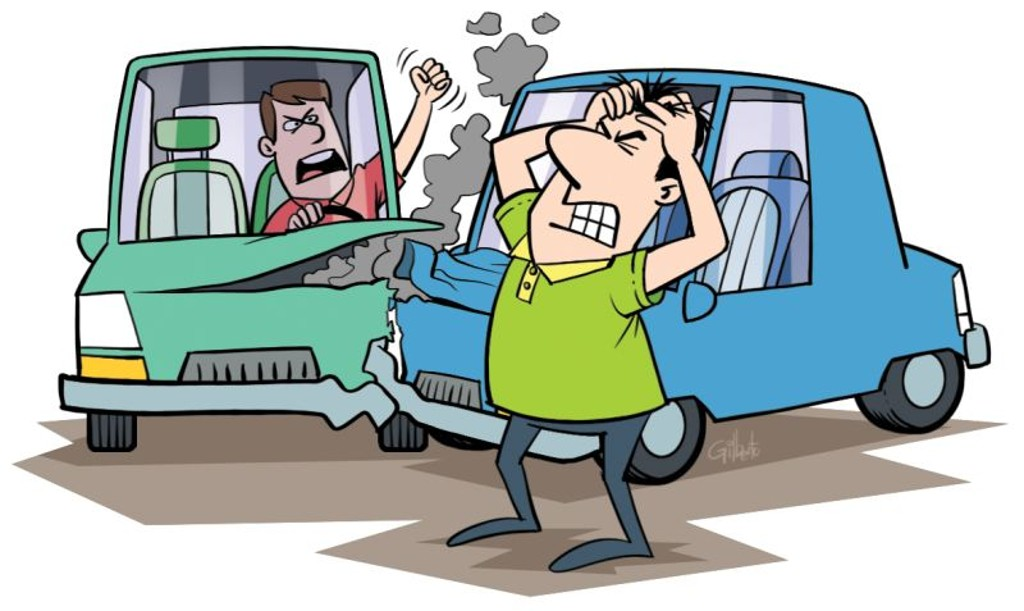
\includegraphics[width=.8\textwidth]{carro-batida.jpg}
			\caption{Batidas de carro já eram frustrantes antes dos carros serem autônomos. Fonte: Gazeta do Povo, internet. }\label{fig:2}
		\end{figure}
		
		E se os carros autônomos fossem rejeitados pela comunidade, seja por medo da insegurança ou da perda de identidade? Será que os carros seriam realmente capazes de interagir com a comunidade de maneira harmoniosa, sem gerar conflitos ou mesmo acidentes?
		
		Além de gerar uma dor de cabeça a mais para as fornecedoras de seguro, o advento dessa nova tecnologia implicaria uma série de valores, que gerariam impactos na sociedade, e podem ser citados com referências ao artigo de \citet{mcbride_ethics_2016}:
		\begin{description}
			\item [Autonomia] Para um computador, nunca existirá autonomia absoluta: ela deve ser balanceada entre humano e máquina - de outro modo, ela buscaria eliminar toda dependência externa, contando apenas com sua sequência de algoritmos e matemática infalível. Entretanto, no momento que essa máquina entrasse em contato com o mundo externo, ela se tornaria exposta, vulnerável e falha. E se ela aprendesse desse mundo, só absorveria mais imprevisibilidade e caos ao seu sistema.
			
			Portanto, a autonomia deve ser equilibrada entre humano e máquina, de maneira que um complemente as falhas do outro, e que se estabeleça a relação de interdependência fundamental entre ambos.
			
			\item [Comunidade] O carro deve estar conectado à comunidade a fim de evitar que se gere um inferno caótico nas ruas da cidade, afinal, ele parte dessa comunidade, que oferece todo o suporte e equipamento dos quais necessitará e na qual irá sempre interagir com pedestres e outros automóveis. Todos os sistemas de conexão devem ser aproveitados em via de compensar a ausência de conexão humana.
			
			É necessária uma visão sistêmica, que reconheça esses carros autoconduzentes em um sistema conectado, aberto aos estudos de relacionamentos complexos. Eles devem agir e exisitr em harmonia com todos os outros elementos que compõem nosso ambiente de convívio pessoal.
			
			\item [Transparência] O projeto deve ser esclarecido para o público com fiel veracidade, sem que nada fique oculto. Os algoritmos utilizados, como são utilizados e suas limitações devem ser compartilhados em sua totalidade, e cada nova alteração ou implementação deve ser de conhecimento público.
			
			As empresas que atuarem nessa área devem levar a sério sua responsabilidade com a comunidade ao comunicar para ela tudo que for relevante com relação ao seu produto.
			
			\begin{figure}[ht]
				\centering
				
\includegraphics[width=.4\textwidth]{pinocchio.png}
				\caption{A omissão ou distorção de aspectos sobre os carros poderia gerar acidentes em massa. Fonte: Pinoquio, internet. }\label{fig:3}
			\end{figure}
			 
			\item [Identidade] A transferência de responsabilidades para máquinas acaba por minar a identidade do homem, tornando-o ignorante e inquestionável. A perda de domínio sobre o automóvel, que hoje em dia muito representa parte da identidade de seu dono, é chocante. Despojado dessa função, o homem se torna incerto quanto a sua própria aptidão, visto que perde sua habilidade no volante para a máquina.
			
			Assim como no filme Wall·e \citep{stanton_walle_2008}, aponta McBride, em que a raça humana se tornou obesa e quase exclusivamente interage com a tela de um computador, o homem perde sua identidade para a máquina, e se torna gradativamente menos humano.
			
			Muitas pessoas se recusariam a passar sua função de motorista para um algoritmo. Ser seu próprio motorista traz ao homem uma sensação de liberdade e independência, e essa perda pode ocasionar alterações emocionais nas pessoas. McBride argumenta, em seu texto, que o homem acaba por se tornar escravo da máquina.
			
			\item [Valores] O que passa a valer mais para nós? A eficiência e valor econômico do carro, ou a excelência humana do motorista? Ele acaba desvalorizado, apenas um objeto a ser carregado de lá para cá?
			
			Evidentemente, o motorista de fato perde seu valor, e é rebaixado para um usuário, ou um passageiro. Cada vez mais, a máquina passa assumir novas funções e agregar mais valor na vida do homem cotidiano. É preocupante imaginar até que ponto isso pode chegar - imaginar o dia em que o homem se tornará subalterno à máquina.
			
			\item [Empatia] McBride aponta que diversas pessoas não aprovariam ser conduzidas por uma máquina por motivos de segurança, pessoais ou estereótipos. Sugere que o engenheiro se mostre dedicado aos medos e expectativas do usuário, que não deve ser tratado como um fator a ser removido do sistema a fim de o tornar mais preciso. O carro deve buscar o humano por trás do volante, apresentar-se como adaptável e sensível, e mostrar-se convidativo.
			
			A transição de sistemas será drástica, e o homem não deve sentir que perdeu por completo seu controle, ele deve sentir que sua vida foi facilitada por essa nova tecnologia, e que a transição será boa. Deve se sentir motivado para acompanhar esse processo e espalhar essa positividade para a comunidade.
			
			\item [Segurança] É inevitável admitir que esse advento tornaria as ruas muito mais seguras. Pesquisas da Waymo \citep{google_-_alphabet_inc._waymo_2009} apontam que em 2014, 1,25 milhão de mortes foram causadas por acidentes de veículos, e esse índice cresce a cada ano que se passa. Estima-se que 94\% desses acidentes envolvem erro ou escolha humana nos EUA. Caso fosse possível eliminar o fator erro humano, as 1,25 milhão de mortes se tornariam apenas 75 mil. A diferença que essa mudança geraria é indescritível, e sem dúvida seria um dos maiores avanços na área da segurança da era contemporânea.
			
			\item [Responsabilidade] E até então, permanece a pergunta: quem seria responsabilizado pelo desempenho desses veículos? Certamente, a resposta mais automática seria a empresa desenvolvedora do algoritmo de condução. No entanto, isso geraria um conflito, já que, ainda mais se tratando de carros independentes, ela não foi explicitamente responsável pelo desenvolvimento do código de funcionamento de seus veículos.
			
			Talvez, ao se tratar de carros conectados, a empresa possa ser responsabilizada, e possa designar uma equipe que se faria responsável por responder pelos acidentes, desenvolver soluções e solucionar falhas do sistema. Outras equipes poderiam ser nomeadas para lidar com testes, estudos, e até mesmo servir como central de atendimento para acompanhar usuários com reclamações e dúvidas.
			
			No entanto, como os carros independentes aprendem por si só e com o humano motorista, os responsáveis imediatos pelos seus erros seriam eles próprios e o usuário. Mas isso dificilmente parece justo, visto que o usuário nada mais fez do que adquirir o produto que prometia trazer-lhe segurança e confiabilidade. Portanto, a questão continua sem resposta, visto que, mesmo se a empresa tomasse as mesmas medidas supracitadas, ainda seria um equívoco transferir a culpa para ela nesse caso.
			
			\item [Confiabilidade] Como o usuário cede sua função de motorista para o carro, espera-se que ele saiba, no mínimo, dirigir com segurança. A vida do passageiro fica a mercê da qualidade do algoritmo que rege o comportamento do veículo, e um erro dele poderia inclusive afetar outras pessoas, como um pedestre, um ciclista ou mesmo outro passageiro. Evidentimente, só deveriam haver carros automotivos no mercado se eles fossem de alta confiabilidade.
			
			Mas não só confiável para esse propósito, o carro também deve se mostrar confiável em sua rota e destino, de forma que seja uma tarefa muito complexa para algum agente externo influenciar-lhes. Caso contrário, eis que surgiria um completamente novo método de sequestro. Até mesmo agentes que só teriam por objetivo coletar informações a respeito da viagem com fins maliciosos podem surgir, entre outras ameaças. O sistema do carro deve ser meticulosamente bem pensado e todas as formas de risco cobertas.
			
		\end{description}
		
	\section{\label{legal}Momento legal ou jurídico}
	
		No quesito jurisdição, a tecnologia abordada geraria uma série de alterações nos artigos que dizem respeito às leis de tráfego e de conduta mobilística. A Lei nº 6.194 \citep{congresso_nacional_lei_1974}, que \emph{dispõe sobre Seguro Obrigatório de Danos Pessoais causados por veículos automotores de via terrestre, ou por sua carga, a pessoas transportadas ou não}, por exemplo, teria de ser sobretudo revisada em seu Art. 8º: \emph{``Comprovado o pagamento, a Sociedade Seguradora que houver pago a indenização poderá, mediante ação própria, haver do responsável a importância efetivamente indenizada"}, afinal, a identidade do sujeito responsável se torna motivo de debate.  Essas leis teriam que incluir a possibilidade de imprevistos ocorridos da imprevisibilidade de um sistema computacional falho. O desenvolvimento desses novos estatutos seria de grande interesse das bancadas automobilíicas, que, sem dúvida, fariam um considerável esforço para tornar o processo ao seu favor.
		
		Certamente as leis e regulações atuais seriam insuficientes para tratar dos conflitos éticos levantados pela tecnologia, como observado acima. Uma nova regulação ideal seria fruto de debates, conferências e dedicação.
		
		Por exemplo, se o carro usufuir da tecnologia de Machine Learning, seria importante promover uma revisão geral do algoritmo regente de seu comportamento, em conjunto com testes de segurança e outras medidas de fiscalização.
		
		Outras leis se tornariam obsoletas, como as que se referem ao Cap. III do Código de Trânsito Brasileiro \citep{congresso_nacional_lei_1997}, referente às normas gerais de circulação e conduta - afinal, o motorista se torna o próprio carro. Essas leis devem transformar-se em requisitos a serem atendidos pelos algoritmos de conduta dos veículos autônomos.
			
		
	\section{\label{praticante}Momento do praticante}
	
		A área de atuação profissional seria altamente remodelada pelo surgimento dessa nova comodidade – num cenário em que prevalecessem apenas os carros autônomos. Algumas profissões seriam desvalorizadas, como motoristas particulares (que se tornariam apenas responsáveis por levar o carro até seu dono e complementar tarefas que o algoritmo computacional fosse incapaz de realizar), outras desapareceriam por completo, como os taxistas e os motoristas de Uber, que seriam substituídos por serviços automáticos de carros-taxi. Empresas inteiras poderiam se extinguir ou lucrar com esse advento: fornecedoras de seguro seriam forçadas a baixar suas taxas (por conta do aumento da segurança no trânsito), reguladoras de trânsito seriam eminentemente reduzidas (ou até mesmo extinguidas), fábricas lucrariam com as ondas de compras da nova tecnologia, empresas desenvolvedoras de novas tecnologias seriam estimuladas… Sobretudo, o maior impacto seria sobre a sociedade em geral, com o dinamismo rotineiro impulsionado pelos carros conectados, de maneira que engarrafamentos desapareceriam e acidentes seriam reduzidos ao mínimo.
		
		\begin{figure}[ht]
			\centering
			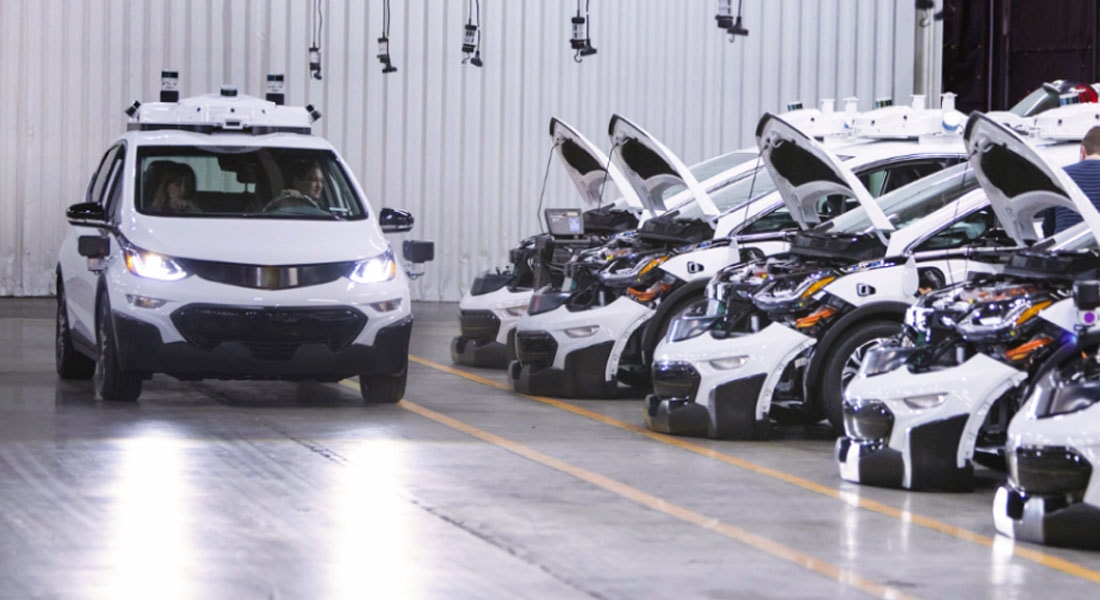
\includegraphics[width=.9\textwidth]{producao-carros.jpg}
			\caption{A General Motors está apostando alto nos carros autônomos, com sua primeira linha de produção em massa de carros autônomos. Fonte: \citet{stylo_urbano_gm_nodate}, internet. }\label{fig:4}
		\end{figure}
		
		Mas sem dúvida, os maiores afetados seriam as empresas automobilísticas, como a Ford, a Hyundai, a Honda, etc. Toda a sua estrutura teria de ser repensada, e o código de conduta estabelecido para seus recém-contratados programadores de algoritmos autômatos. Teriam de ser levantados vários debates acerca da ética relacionada a possíveis futuros eventos conflitantes, de maneira a estipular o melhor código de conduta o possível.
		
	\section{\label{conlusoes}Conclusões}
		
		Evidentemente, tratar de carros autônomos é tratar de um assunto extremamente complexo e que envolve uma série de aspectos sociais, legais, éticos e econômicos. A análise promovida nesse artigo meramente objetiva iniciar uma reflexão ética acerca do papel do motorista na sociedade e como deve ser tratado esse progresso tecnológico.
		
		No que envolve o debate carro conectado e carro independente, não somente o autor do artigo base, \citet{mcbride_ethics_2016}, mas também o autor desse mesmo artigo concordam que uma melhor opção sem dúvida seria um carro integrado e conectado - mesmo que talvez apenas por alguns anos, ou décadas, até que a tecnologia de machine learning se torne definitivamente confiável ou seja ainda superada por outra emergente tecnologia, como a Deep Learning.
		
		É provável que a única maneira de buscar a solução para esses dilemas morais levantados seja por meio da tentativa e erro. No entanto, não se deve descartar o momento de reflexão jamais, pois ele é de suma importância para qualquer processo de pesquisa e extensão de conhecimentos. E nesse caso específico ainda é sim possível obter algumas conclusões importantes, como o desenvolvimento de novas leis e códigos de conduta, novas estratégias de alinhamento econômico, e ainda outras possibilidades não abordadas nesse documento.
		
		O importante é que essa tecnologia não deve surgir como uma novidade inesperada na sociedade, e cada cidadão já deve ter pleno conhecimento de seu funcionamento e suas vantagens antes de começar a consumir essa inovação. 
		
	\bibliographystyle{pt-plainnat}
	\bibliography{InfoSoc20172}
	
\end{document}
